\documentclass[main.tex]{subfiles}

\begin{document}
\section{Question II}\label{sec:question II}

\subsection{Problem}
Solve the CarRacing-v2 gym environment using PPO algorithm
\subsection{Solution}

To solve the problem presented by the CarRacing-v2 environment we chose to implement an advanced and highly optimized version of the Proximal Policy Optimization algorithm freely inspired by the proposed Stable-Baseline3 library following the indications of the paper \cite{huang2022a2cspecialcaseppo} and blog \cite{shengyi2022the37implementation}.

The choice to implement the PPO algorithm was guided by the papers made available. From the paper \cite{schulman2017proximalpolicyoptimizationalgorithms} regarding the PPO it was clear that the A2C algorithm, although adequate to solve the problem in question, is not the most efficient and effective for a complex environment such as that of CarRacing, therefore it was excluded a priori. The DDQN+PER algorithm, on the other hand, was not taken into consideration given the objective limitation of the DDQN algorithm even if improved with the Prioritized Experience Replay buffer which improves its convergence rate and makes DDQN applicable even to complex problems \cite{schaul2016prioritizedexperiencereplay}. The TRPO was not chosen given the possibility of implementing the PPO algorithm which, compared to the TRPO, avoids explicitly calculating the particularly complex Trust Region \cite{schulman2017proximalpolicyoptimizationalgorithms}. Finally, the World Models, although known to have great potential in multiple environments, \cite{https://doi.org/10.5281/zenodo.1207631} was deemed excessively advanced for the task in question, therefore the final choice fell on Proximal Policy Optimization algorithm.

\subsubsection{Analysis of the problem}
At first inspection, the problem appears to lack the defining components of a Markov decision process, rendering standard reinforcement learning frameworks inapplicable. In particular, essential constructs such as well-defined policies, value functions, and Bellman optimality equations do not seem to be meaningfully expressible in this setting. 

This problem is caused because by observing the position of the car in a single frame of the scene, we cannot infer any information about the current state of speed, direction of movement, etc..., which is necessary to understand how the car will move and, consequently, the next state of the system.

\begin{figure}[H]
	\centering
	\includegraphics[width=0.4\linewidth]{f1.png}
	\caption{Single frame video of environment}
	\label{fig:car.racing.env}
\end{figure}

Fortunately, in this case, the environment itself graphically provides us with additional information, indicating the velocity and acceleration/deceleration values at the bottom of the image in the form of colored bars. The additional information displayed is sufficient to retrieve the information needed to make a single video frame valid for predicting the next state, thus making the basic problem perfectly MDP-like.

\begin{figure}[H]
	\centering
	\includegraphics[width=0.5\linewidth]{f1_2.png}
	\caption{Detail of the sensors}
	\label{fig:car.racing.env.sensors}
\end{figure}

\subsubsection{overview of innovations}
The innovations introduced compared to the classic PPO implementation can be summarized as follows:

\begin{itemize}
	\item Use of parallel environments in the rollout phase to reduce variance and increase the algorithm's convergence speed (more exploration and episodes for the same time point)
	
	\item Introduction of additional clipping terms in the loss formulation for greater stability
	
	\item Orthogonal weights initialization
	
	\item Annealing method for learning rate
	
	\item Advance Buffering Methods
	
	\item Async environments implementation (for high parallelization)
	
	\item Default use of the GAE algorithm
	
\end{itemize}

This set of implementation details have led to remarkable results without distorting the basic fundamental idea.



\subsubsection{Weights Initialization}
As confirmed by the studies \cite{Engstrom2020Implementation} and \cite{andrychowicz2021what}, using the orthogonal initialization method of the weights $\theta_\pi $ and $\theta_v$ allows for qualitatively better results, quantified in a better convergence rate of the algorithm, compared to the standard mechanism implemented by individual machine learning libraries (e.g., Xavier). The Orthogonal method guarantees these improvements, unlike other methods, regardless of the depth of the neural network.

\begin{listing}[H]
	\centering
	\caption{Wrapper function code for orthogonal initialization of weights and biases } 
	\label{codice:init}
\begin{minted}[frame=lines, framesep=2mm, baselinestretch=1.2, bgcolor=bg, linenos]{python}
def layer_init_(layer, std=np.sqrt(2), bias_const=0.0):
	torch.nn.init.orthogonal_(layer.weight, std)
	torch.nn.init.constant_(layer.bias, bias_const)
	return layer
\end{minted}
\end{listing}
\subsubsection{Rollout Environments specifications}
Among the advanced specifications implemented, the use of parallel environments is certainly the most advanced, allowing for a varied and exhaustive exploration of the environment.

Using the advanced features provided by the Gymnasium environment we can easily create a vector $E$ environment composed of $N$ independent asynchronous CarRacing-v2 environments through the use of the Async option which allows true parallelism across multiple processors ('cores') ensuring high throughput during the rollout phase.

\begin{figure}[H]
	\centering
	\includegraphics[width=0.4\linewidth]{f2.png}
	\caption{Conceptual representation of the $E$ environment running on a multi-core CPU}
	\label{fig:envs}
\end{figure}

Generally, modern processors of the last few years adopt an octa-core configuration (8 processors) therefore 8 was chosen as the number of parallel environments obviously increasing this value significantly improves the results.

\begin{listing}[H]
	\centering
	\caption{Initialization of environments} 
	\label{codice:init_envs}
	\begin{minted}[frame=lines, framesep=2mm, baselinestretch=1.2, bgcolor=bg, linenos]{python}
# Vectorized Env E ####################################
self.envs = gym.make_vec(
'CarRacing-v2',             # Type enviroment
num_envs=self.N,            # Number parallel envs
vectorization_mode="async", # Async mode
continuous=self.continuous, # Discrate/Continuos env
render_mode='rgb_array'     # 2D RGB array
)
#######################################################
	\end{minted}
\end{listing}

\subsubsection{Neural Network}

The optimal value function $V_\theta$ and the optimal policy $\pi_\theta$ in the PPO algorithm are estimated using parameterized neural network models optimized via gradient descent (SGD or Adam). Since the observation returned by the environment is an RGB image and classical neural networks expect a numerical vector of features as input, it is necessary to use some kind of encoder that encodes the image into a feature vector that can be processed by a fully connected neural network.

\begin{figure}[H]
	\centering
	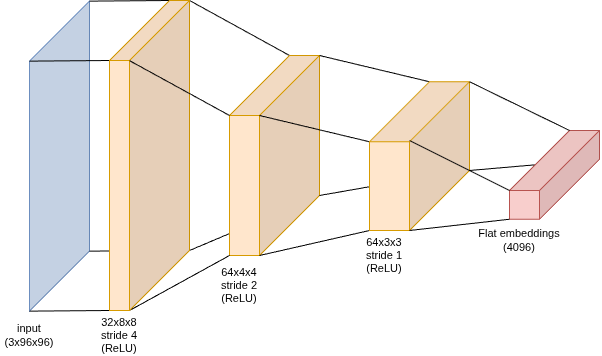
\includegraphics[width=0.8\linewidth]{f3.png}
	\caption{Observation encoder architecture}
	\label{fig:img_encoder}
\end{figure}


To this end, among the various available options, we adopted a convolutional neural network (CNN) as the encoder, a standard choice for extracting embeddings from visual data. Since it is also a neural model, it will be optimized during training together with the $V_\theta$ and $\pi_\theta$ estimators, making the learning process more linear and consistent.

The processed embeddings are then passed to two independent deep neural networks that estimate the policy and the Value function, respectively. The output of the networks will be those predicted by the estimated functions.

\begin{figure}[H]
	\centering
	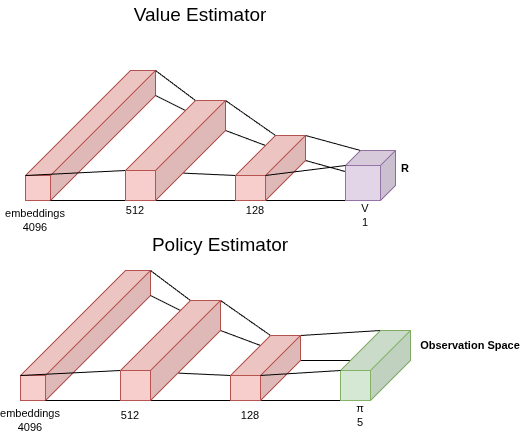
\includegraphics[width=0.6\linewidth]{f4.png}
	\caption{Observation encoder architecture}
	\label{fig:estimators}
\end{figure}

The structures of the CNN network and the linear network as well as the definition of the individual layers were inspired by the literature on the subject.

\subsubsection{Buffering}
The use of a replay buffer is one of the distinctive and fundamental features of PPO. The buffer is the tool for calculating key quantities such as the advantage (normal or via GAE) and the target return (RT), which will contribute to the gradient calculation during the network weight optimization phase.

\begin{listing}[H]
	\centering
	\caption{Initialize buffers} 
	\label{codice:buffers}
	\begin{minted}[frame=lines, framesep=2mm, baselinestretch=1.2, bgcolor=bg, linenos]{python}
# buffer D ########################################
obs_buf = torch.zeros((self.M, self.N, 3, self.img_size[0], self.img_size[1]))
reward_buf = torch.zeros((self.M, self.N))
values_buf = torch.zeros((self.M, self.N))
logp_buf = torch.zeros((self.M, self.N))
action_buf = torch.zeros((self.M, self.N))
done_buf = torch.zeros((self.M, self.N))
##########################################
	\end{minted}
\end{listing}

The implementation does not explicitly construct a two-dimensional buffer as described in the reference paper. Instead, for ease of implementation, the buffer is realized as a collection of independent, parallel buffers, each of size $(N \times M)$
\subsubsection{Rollout Procedure}

The PPO rollout procedure consists of generating a series of trajectories $(o_t, r_t, v_t, d_t, d_{t+1}, o_{t+1})_{i=1}^{N}$ from the $N$ environments for M time instants and then storing them within the appropriate buffers. Thanks to the use of the vectorized and parallel environment provided by gymnasium, the entire rollout procedure is executed efficiently in batch. The trajectories collected, as already stated, will then be used to calculate the advantage and the Target return value as well as in the subsequent learning phase.

\begin{listing}[H]
	\centering
	\caption{Roll-out procedure} 
	\label{codice:rollout_1}
	\begin{minted}[frame=lines, framesep=2mm, baselinestretch=1.2, bgcolor=bg, linenos]{python}
for t in range(self.M):

	# cache
	envs_next_o = self.o_next # (num_envs x (3, 96, 96))
	envs_next_d = self.d_next # (num_envs x 1)
	####################################################
	# prepare batchs
	
	# actor use current estimated policy
	curent_action, current_action_logp, current_value = self._act(envs_next_o)
	
	# remove batch 
	current_value = torch.squeeze(current_value, dim=1)
	
	#rollout phase
	
	# parallel execution (True parallel)
	o, r, terminated, truncated,  infos = self.envs.step(curent_action.numpy())
	dones = terminated | truncated
	np_dones = np.array(envs_next_d, dtype=np.float32)
	\end{minted}
\end{listing}

The buffer's operating logic is to simultaneously make available the information for the old policy used during the rollout phase and the new one estimated during the learning phase. For this reason, a caching mechanism is also provided to retain the past values, which would otherwise be erased by subsequent rollouts. The code below handles this situation, along with other techniques derived from the vectorized environment.

\begin{listing}[H]
	\centering
	\caption{Update buffers} 
	\label{codice:rollout_2}
	\begin{minted}[frame=lines, framesep=2mm, baselinestretch=1.2, bgcolor=bg, linenos]{python}
for t in range(self.M):
	
	# cache
	envs_next_o = self.o_next # (num_envs x (3, 96, 96))
	envs_next_d = self.d_next # (num_envs x 1)
	####################################################
	# prepare batchs
	
	# actor use current estimated policy
	curent_action, current_action_logp, current_value = self._act(envs_next_o)
	
	# remove batch 
	current_value = torch.squeeze(current_value, dim=1)
	
	#rollout phase
	
	# parallel execution (True parallel)
	o, r, terminated, truncated,  infos = self.envs.step(curent_action.numpy())
	dones = terminated | truncated
	np_dones = np.array(envs_next_d, dtype=np.float32)
	
	# store all data in buffers
	o = self.to_tensor(o)
	self.o_next = o
	self.d_next = torch.from_numpy(np_dones).float()
	################################################
	
	# store in buffers
	obs_buf[t]  = envs_next_o
	reward_buf[t] = torch.from_numpy(r).float()
	action_buf[t] = curent_action.long()
	logp_buf[t] = current_action_logp
	values_buf[t] = current_value
	
	# recover last observatio when env is reset
	for i in range(len(dones)):
	if dones[i]:
	if "final_observation" in infos:
	obs_buf[t][i] = self.to_tensor(infos["final_observation"][i])
	self.o_next[i] =  o[i]
	print(f"Reset env {i}, term_normal={terminated[i]}")
	
	#############################################################
	\end{minted}
\end{listing}

Finally, all that remains is to calculate the benefit and expected return terms using the terms stored in the buffers. The most computationally efficient method to calculate the GAE value is to use the backward iterative definition:

\begin{equation}
	\label{GAE}
	\hat{\mathcal{A}}_{t}^{GAE} = \delta_t + \gamma\hat{\mathcal{A}}_{t + 1}^{GAE}
\end{equation}

where:

\begin{equation}
	\delta_t = r_{t+1} + \gamma V(s_{t+1}) - V(s_t) 
\end{equation}

is TD-Error.

For the final step we set $\hat{\mathcal{A}}_{T}^{GAE} = v_\theta(d_{next})$, then the \ref{GAE} definition applies from timestamp $T$ to $0$.
\begin{listing}[H]
	\centering
	\caption{GAE computation} 
	\label{codice:GAE}
	\begin{minted}[frame=lines, framesep=2mm, baselinestretch=1.2, bgcolor=bg, linenos]{python}
for t in reversed(range(self.M)):
	if t == self.M - 1: # start from last timestamp
	next_non_terminal = 1.0 - self.d_next 
	next_val = last_value
	else: # applay recursive definition
	next_non_terminal = 1.0 - done_buf[t+1]
	next_val = values_buf[t+1]
	
	# compute iter.
	delta = reward_buf[t] + self.gamma * next_val * next_non_terminal - values_buf[t]
	last_gae_lam = delta + self.gamma * self.gae_lambda * next_non_terminal * last_gae_lam
	advantages[t] = last_gae_lam
	\end{minted}
\end{listing}
Using the GAE formulation for calculating the benefit, the target return can be calculated simply as follows:

\begin{listing}[H]
	\centering
	\caption{Target Return computation} 
	\label{codice:TD}
	\begin{minted}[frame=lines, framesep=2mm, baselinestretch=1.2, bgcolor=bg, linenos]{python}
target_return = advantages + values_buf # TD
	\end{minted}
\end{listing}




\subsubsection{Learning Procedure}
In the learning phase, the PPO algorithm exploits the knowledge about the behavior of the environment acquired during the rollout phase to update the estimate of the policy as well as the value function. The most relevant part in the learning phase is the calculation of the loss value determined by three loss values.

The first loss term is called clipped or surrogate policy loss and are composed of two principal terms: the Ratio and estimated advantage. The Ratio expresses how much the currently estimated policy (learning) varies compared to the previous one (rollout). It can be computed as follow:
\begin{listing}[H]
	\centering
	\caption{Target return computation respect GAE value} 
	\label{codice:tr}
	\begin{minted}[frame=lines, framesep=2mm, baselinestretch=1.2, bgcolor=bg, linenos]{python}
policy_logits, current_values = self.forward(obs)
current_values = current_values.flatten()
dist = torch.distributions.Categorical(logits=policy_logits)
current_policy_logp = dist.log_prob(action)
ratio = torch.exp(current_policy_logp - logp)
	\end{minted}
\end{listing}
 
Using the Current Policy probabilities (calculated via the Actor network), calculate the ratio between the old buffered policy and the current one (note that in the first iteration the ratio will be 1, subsequent weight updates will make this value different than 1). The advantage used is instead the one estimated during the rollout phase (using the Value Function).

\begin{listing}[H]
	\centering
	\caption{Computation for Policy} 
	\label{codice:ratio}
	\begin{minted}[frame=lines, framesep=2mm, baselinestretch=1.2, bgcolor=bg, linenos]{python}
policy_ratio = advantage * ratio
	\end{minted}
\end{listing}

This loss term determines how to update the probability of actions taken during the rollout. It is constrained in two ways: first by using a probability ratio to enable multiple updates on collected data, and second by clipping this ratio within a neighborhood of $\epsilon$ to prevent destructive policy updates.
\begin{listing}[H]
	\centering
	\caption{Computation surrogate policy loss} 
	\label{codice:policy_loss}
	\begin{minted}[frame=lines, framesep=2mm, baselinestretch=1.2, bgcolor=bg, linenos]{python}
policy_clip = advantage * torch.clamp(ratio, 1 - self.epsilon, 1 + self.epsilon)
policy_loss = -torch.min(policy_ratio, policy_clip).mean()
	\end{minted}
\end{listing}

The Value Loss is calculated by first constraining the current value estimate so that it does not deviate excessively from the previous rollout value (using a clipping mechanism similar to the policy's). The final loss term is then computed as the Mean Squared Error (MSE) between this constrained (clipped) value estimate and the target return obtained during the rollout.

\begin{listing}[H]
	\centering
	\caption{Computation Clipped Value Loss} 
	\label{codice:value_loss}
	\begin{minted}[frame=lines, framesep=2mm, baselinestretch=1.2, bgcolor=bg, linenos]{python}
# Value loss
critic_loss_clip = value + torch.clamp(current_values - value, -self.clip_v, self.clip_v) 
critic_loss = F.mse_loss(target_return, critic_loss_clip)
	\end{minted}
\end{listing}

Finally, the last term to discuss concerns Entropy. The entropy term is an additional value that allows us to account for the policy's need for exploration. Without this term, the policy would risk "premature convergence", becoming deterministic too early and getting stuck in local optima instead of exploring better strategies.

\begin{listing}[H]
	\centering
	\caption{Computation Entropy Loss} 
	\label{codice:entropy_loss}
	\begin{minted}[frame=lines, framesep=2mm, baselinestretch=1.2, bgcolor=bg, linenos]{python}
# entropy term
entropy_loss  = -dist.entropy().mean()
	\end{minted}
\end{listing}

The general behavior of this term is expected to be quite high in the first iterations of the algorithm and then gradually decay as the policy estimate improves.

Finally, the sum of all the analyzed terms determines the total loss value. 

\begin{listing}[H]
	\centering
	\caption{Target return computation respect GAE value} 
	\label{codice:loss}
	\begin{minted}[frame=lines, framesep=2mm, baselinestretch=1.2, bgcolor=bg, linenos]{python}
loss = policy_loss + self.c1 * critic_loss + self.c2 * entropy_loss
	\end{minted}
\end{listing}

Note the two additional factors $c1$ and $c2$, which respectively regulate the influence of the value loss term and the entropy term, allowing for precise control of the optimization step and the entropy contribution to the total loss value.

\subsubsection{Hyper-parameters and Results}
\begin{table}[t]
	\centering
	\caption{PPO hyper-parameters}
	\label{tab:ppo_hyperparameters_columns}
	\resizebox{\textwidth}{!}{
		\begin{tabular}{ccccccccccccccc}
			\hline
			$N$ & $M$ & $K$ & $I$ & Img size & $\epsilon$ & $\gamma$ & $\lambda$ & $\|\nabla\|_{\max}$ & $\epsilon_v$ & $c_2$ & $c_1$ & Mean Reward \\
			\hline
			8 & 512 & 5 & 500 & $96\times96$ & 0.2 & 0.99 & 0.95 & 0.5 & 0.2 & 0.02 & 0.5 & 920 $\pm$ 20 \\
			\hline
		\end{tabular}
	}
\end{table}
The hyperparameters tested are the recommended ones obtained by analyzing several PPO jobs with different environments. The results obtained with these hyperparameters are very satisfactory, with an average reward around 920, confirmed in rendering mode by a perfect execution of the generated path.


\subsubsection{Conclusions}

The implemented version of the PPO algorithm turns out to be optimal for the solved problem, achieving exceptional results on a par with more complex techniques such as the word model. This proves that the choice of using the PPO was adequate for the proposed task as already analyzed in the introduction.

\end{document} 